\documentclass[a4j,twoside,openright,11pt]{jsarticle}
%
\usepackage{amsmath,amssymb}
\usepackage{bm}
\usepackage{graphicx}
\usepackage{ascmac}
\usepackage{listliketab}
\usepackage{url}
\usepackage{listings}

\setlength{\textwidth}{15.92cm}
\setlength{\oddsidemargin}{0mm}
\setlength{\evensidemargin}{0mm}
\setlength{\topmargin}{-1cm}
\setlength{\textheight}{23.5cm}
\setlength{\footskip}{18mm}

%\pagestyle{plain}

\begin{document}
\begin{screen}
\huge
\begin{center}
{\bf 機械工学実験\\NC工作機械の精度誤差計測}\\
\end{center}

\normalsize
\begin{flushright}
九州工業大学 機械知能工学科 機械知能コース  坂本 悠作\\学籍番号:13104069 \hspace{0.2in}実験日 2015年4月15日  提出日 2015年5月8日
\end{flushright}
\end{screen}


\section{実験目的}
NC工作機械(NC旋盤)を使用し、加工前後の被削物の寸法を測定することで、工作機械の操作、精度評価、検証方法について学習する
\section{原理}
次に示すように、計測して得られた誤差の分だけ切り込み量を減らして加工することで、目標とする加工精度に調節する。
\begin{figure}[htbp]
\begin{center}
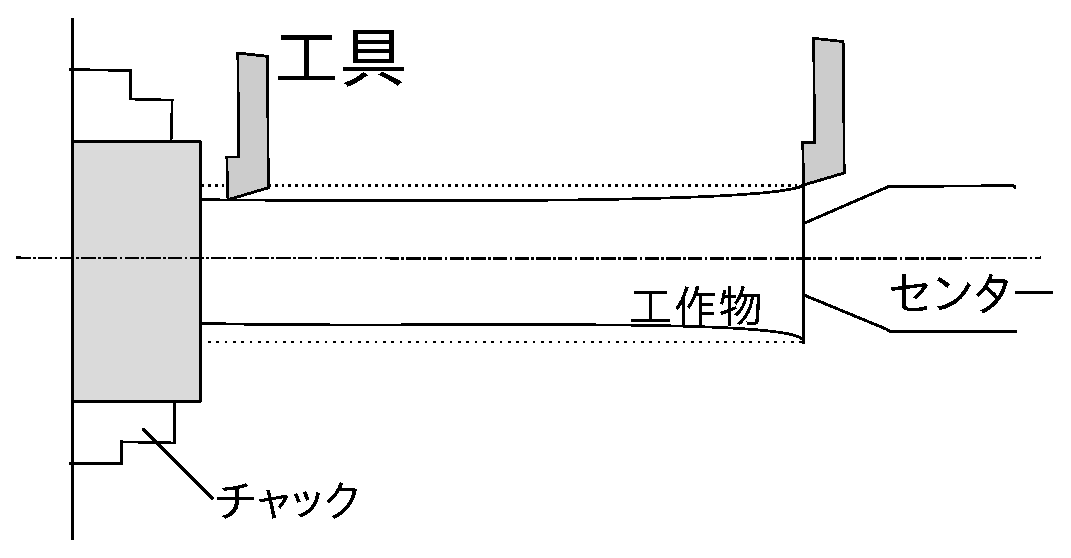
\includegraphics[width=12cm]{hoseimae.eps}
\end{center}
\caption{補正前の刃物経路}
\end{figure}
\begin{figure}[htbp]
\begin{center}
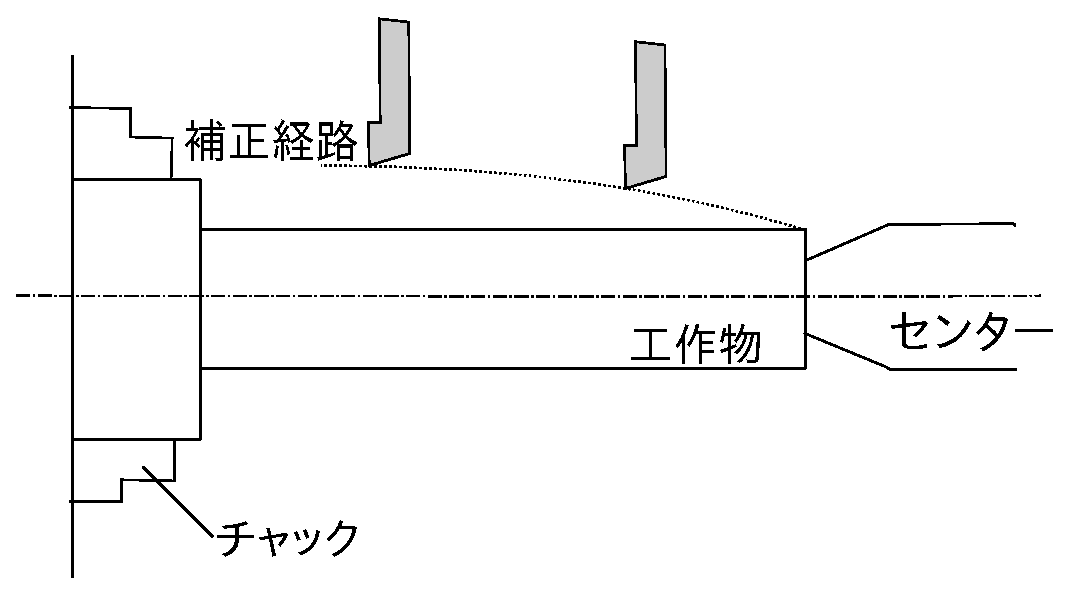
\includegraphics[width=12cm]{hoseigo.eps}
\end{center}
\caption{補正後の刃物経路}
\end{figure}
これにより誤差を完全に無くすことはできないが、目的の精度に近づけることができる。
\newpage
\section{実験方法}
\subsection{実験手順}
\begin{enumerate}
\item 加工物に対し1mmの切り込みを与え、補正なしで1回加工を行う。加工距離は最長で200mmまで。
\item 電気マイクロメータを取り付け、Z軸方向に走査させて加工物の直径寸法を20mmごとに測定する。データは表示器の値を読み取り、記録用紙に記録する
\item 得られたデータをもとに、NC命令を修正し、補正加工を行う。
\item 再度電気マイクロメータにより計測を行う。
\item 補正加工前後の形状誤差精度を比較して、加工誤差について計測する
\end{enumerate}

\section{考察}
\subsection{用語}
\begin{itemize}
\item サーボ機構\\
  サーボ機構はエンコーダによる速度や位置のフィードバックによって目標とする位置や速度を実現する制御機構。
\item ボールねじ\\
  ボールねじは、回転運動を直線運動に変換する機械要素で、UFOキャッチャーのアームにも使用されている。ボールを用いて摩擦係数を低くしているので、ボールを絶やさないために回収する機構が必要不可欠となり、値段も2万円以上となる。しかし精密機械には必要な要素でもある。\\
  ボールねじの組み合わせ方式の種類には、シングルナット方式、ダブルナット方式、インテグラルナット方式があり、与圧区分に応じて使い分ける必要がある。\\
  ボールねじはナット内にゴミや異物が挿入すると摩耗が速く進む傾向にあるため、ジャバラやカバーを取り付けて防塵対策をする必要がある。\\
  ボールねじの製造法には転造と研削があり、転造の方が寿命が長く、安くて加工硬化もあるが、研削程の精度は出せない。
\item 電気マイクロメータ\\
  電気マイクロメータは、差動トランス(Differential Transfer)の原理を用いた測定器で、精度によっては0.01$\mu$mまでの測定が可能である。差動トランスとは、1次コイル、2次コイル、鉄心で構成されており、1次コイルに交流電流を流すと、二次コイルに伝えられる電力が線形性を示すことから、一般に使用されている。
\end{itemize}

\subsection{実験結果のまとめと比較}
\begin{itemize}
\item 材質:S35C
\item 工具:超硬(P10)チップ
\item 工具回転数(n):1000rpm
\item 測定位置:端面から20mm毎に100mmまで
\item 切削速度(V):150m/min
\item 送り速度(f):100mm/min
\item 切削状態:ドライ切削
\end{itemize}
\begin{table}[htb]
\begin{center}
  \caption{実験結果:電気マイクロメータ}
  \begin{tabular}{|l||c|c|} \hline
    距離    &補正無し($\phi$=51mm) &補正あり($\phi$=50mm)\\
\hline
    0(端面位置) &0                   &0\\
    20mm        &0.009               &-0.002\\
    40mm        &0.011               &-0.001\\
    60mm        &0.013               &-0.001\\
    80mm        &0.014               &0\\
    100mm       &0.015               &0\\
\hline
    最大値      &0.015               &-0.002\\
\hline
  \end{tabular}
\end{center}
\end{table}

上の結果は、センターから距離が離れるとたわみによって加工誤差が生じてしまうため、補正を行うことで誤差を小さく抑えた結果である。誤差最大値をみると-0.002mmの誤差が生じているが、軸直径の精度が良ければどのJIS規格も満たすことが可能である精度である。補正によって得られる精度向上は十分に得られていると取れる。

\newpage

\begin{table}[htb]
\begin{center}
  \caption{実験結果:マイクロメータとノギスの測定結果}
  \begin{tabular}{|l||c|c|c|c|} \hline
    &マイクロメータ&マイクロメータ&ノギス&ノギス\\
    回数 &補正無し($\phi$=51mm) &補正あり($\phi$=50mm)&補正無し($\phi$=51mm) &補正あり($\phi$=50mm)\\
\hline
    1回目 &50.968               &49.975 & 50.96&49.99 \\
    2回目 &50.963               &49.981 & 50.94&49.98 \\
    3回目 &50.965               &49.982 & 50.96&49.99 \\
\hline
    平均値&50.965               &49.979 &50.95 &49.99 \\
\hline
  \end{tabular}
\end{center}
\end{table}

それぞれの平均値を使って誤差を比較して見ると、以下のようになる。\\
また、直径の大きさの違いによる誤差の大きさは、端面を測定しているという条件から考慮しないものとする。
\begin{eqnarray}
(マイクロメータ補正なし誤差)51 - 50.965 &=& 0.035mm\nonumber\\
(マイクロメータ補正あり誤差)50 - 49.979 &=& 0.021mm\nonumber\\
(ノギス補正なし誤差)51 - 50.95 &=& 0.05mm\nonumber\\
(ノギス補正あり誤差)50 - 49.99 &=& 0.01mm\nonumber
\end{eqnarray}
結果を見ると、明らかに誤差が小さくなっていることがわかる。

\subsection{考えられる誤差要因}
チャックの部分に誤差があると考えると、今回使用したNC旋盤は3つ爪チャックで固定、かつセンターで両側固定であるので、掴む部分の部材の真円度や軸に対する直角性が必要になってくる。\\
その他の理由は工作機械そのものの精度によると考えられる。

\subsection{NCの振動制御}
振動はあらゆる要素で発生する可能性がある。今回のNC工作機械では、ボールねじのボール回収時の振動であったり、共振周波数における振動だったりする。\\
\par
機械・建築の部材構造で頻繁に使用されているものを以下に示す。
\begin{enumerate}
\item トラス構造\\
トラス(Truss)構造は、三角形を基本単位としてその集合体で構成する構造様式。
部材の接点をピン接合とし、木や鋼鉄が用いられることが多い。部材及び接合部を剛体とみなして解析する。このトラス構造がなぜ用いられているかというと、爪楊枝を思い浮かべてもらいたい。爪楊枝に横からの力を加えると、すぐに折れてしまうが、引張・圧縮の力を加えて爪楊枝を破壊するのは非常に大きな力が必要となる。このように、部材に引っ張り、圧縮だけの力が加えられれば構造的に破壊されにくくなる。これを利用したものが、トラス構造である。
\item ハニカム構造\\
ハニカム構造は、英語で書くと(honeycomb)と書く。これは、蜂の巣のような6角形のものを基本構造とするものである。確かに構造的にはトラス構造のほうが強度的には耐えられるが、衝撃の吸収や熱の遮断には非常に有効な構造になる。この構造は軽量化・制振等の効果を生み出すので、様々な分野で用いられている。
\item ラーメン構造\\
ラーメン構造は、長方形に組まれた骨組み(部材)の各接合箇所を剛接合したものをいう。接合部が非常に頑強なので、地震荷重や風荷重に耐えることができる。建築分野では最も多く用いられている構造である。
\item 壁式構造\\
柱と梁の代わりに耐力壁で荷重を支える構造である。鉄筋クリートの壁だけで構成されているため、室内にスッキリした空間を作ることができる。
\item 架橋式構造\\
これと比較されるのが式構造である。柱と梁で床や壁を支える方法のこと
\end{enumerate}
このように、構造によって振動を吸収するという方法があるが、他にもDCサーボモータの制御であったり、除振装置の使用であったり、加振力自体を低減させる方法であったりする。

\section{参考文献}
\begin{itemize}
\item \url{http://water.jfe-advantech.co.jp/technical/knowledge/transformer/principle.php}
\item \url{http://blog.mukae.co.jp/article/33356305.html}
\item \url{http://www.nttd-es.co.jp/products/e-learning/e-trainer/trial/nc/nc_dnc.htm}
\item \url{http://www.kuroda-precision.co.jp/products/FA/BS_QandA/bal0217.htm}
\item 精密位置決め機構設計 工業調査会 大塚二郎ら
\end{itemize}

\end{document}